\documentclass{article}
\usepackage[utf8]{inputenc}
\usepackage[brazil]{babel}
\usepackage{minted}
\usepackage{graphicx}
\usepackage{hyperref}
\hypersetup{
    colorlinks=true,
    linkcolor=blue,
    filecolor=magenta,      
    urlcolor=blue
}

\title{INE5429 - Let's Encrypt \\ Relatório}
\author{Gustavo Kundlatsch}
\date{\today}

\begin{document}

\maketitle

\section{Introdução}

O Let's Encrypt é uma autoridade de certificação fundada pelo Internet Security Research Group. Foi lançada em abril de 2016 com o objetivo de oferecer gratuitamente certificados de criptografia TLS X.509. Nessa relatório, será mostrado como foi criado um servidor de testes que utiliza de forma automática certificados Let's Encrypt.

\section{Ferramentas}

Algumas ferramentas são necessárias para utilizar certificados da Let's Encrypt. Primeiro, é necessário ter um domínio registrado. É possível obter um domínio gratuitamente através do \href{https://education.github.com/pack}{GitHub Student Pack} (é necessário possuir uma conta de estudante no GitHub, que pode ser confirmada com o email institucional da sua universidade). Para realizar o trabalho proposto, foi cadastrado um domínio na plataforma \href{https://www.namecheap.com/}{NameCheap}.

Além do domínio, é preciso utilizar um serviço de hospedagem para que possamos colocar nosso servidor em produção. Para isso, foi utilizado o serviço Elastic Beanstalk do Amazon Web Services, que permite hospedarmos nossa aplicação de maneira simples e realizar as manipulações que precisamos (como será visto mais tarde).

Para desenvolver o servidor, foi utilizada a linguagem JavaScript com o runtime Node.js, muito comum no desenvolvimento de servidores. O framework express foi usado para criar as rotas da aplicação. O código utilizado será disponibilizado na próxima seção.

Por fim, para gerar o certificado que será distribuído, foi utilizado o \href{https://certbot.eff.org/}{Certbot}, conforme indicado como meio mais recomendado para usuários com acesso ao shell no próprio site da Let's Encrypt.

\section{Desenvolvimento}

Para criar um serviço que utiliza a certificação da Let's Encrypt, primeiro é necessário instalar o Certbot para gerar essa certificação. Em uma distribuição Linux baseada em Debian (como o Ubuntu ou Mint), que utilizam o gerenciador de pacotes APT, é possível instalar o Certbot com os seguintes comandos:

\begin{minted}{shell}
    sudo add-apt-repository ppa:certbot/certbot
    sudo apt-get update
    sudo apt-get install certbot
\end{minted}

Antes de criar o certificado, inicie sua aplicação node, para que já tenhamos a base necessária:

\begin{minted}{shell}
mkdit letsencypt
cd letsencrypt
npm init
\end{minted}

Digite as informações solicitadas, como nome do pacote, versão e autor. Depois disso, já podemos começar a gerar o certificado com o Certbot:

\begin{minted}{shell}
    sudo certbot certonly --manual
\end{minted}

Com o início da geração do certificado, as seguintes mensagens aparecerão no terminal:

\begin{minted}{shell}
$ sudo certbot certonly --manual
[sudo] senha para <pc>: 
Saving debug log to /var/log/letsencrypt/letsencrypt.log
Plugins selected: Authenticator manual, Installer None
Please enter in your domain name(s) (comma and/or space separated)
(Enter 'c' to cancel): 
\end{minted}

Para continuar, basta digitar o domínio que foi registrado, e confirmar que aceita que o IP da máquina utilizada seja salvo de maneira pública:

\begin{minted}{shell}
Obtaining a new certificate
Performing the following challenges:
http-01 challenge for <host>

- - - - - - - - - - - - - - - - - - - - - - - - - - - - - - - - -
NOTE: The IP of this machine will be publicly logged as having
requested this certificate. If you re running certbot in manual
mode on a machine that is not your server, please ensure you re 
okay with that.

Are you OK with your IP being logged?
- - - - - - - - - - - - - - - - - - - - - - - - - - - - - - - - - 
(Y)es/(N)o: Y
\end{minted}

Com isso, você vai receber uma mensagem informando uma `a-string' e uma `a-challange':

\begin{minted}{shell}
- - - - - - - - - - - - - - - - - - - - - - - - - - - - - - - - -
Create a file containing just this data:

http://<host>/.well-known/acme-challenge/a-string

And make it available on your web server at this URL:

a-challange

- - - - - - - - - - - - - - - - - - - - - - - - - - - - - - - - - 
Press Enter to Continue

\end{minted}

O enter pode ser precionado, mas ao invés de continuar o processo, você deve criar uma pasta `.well-known', e dentro dela uma pasta `acme-challenge'. Dentro da acme-challange, crie um arquivo com o nome mostrado no lugar de a-string, e dentro desse arquivo cole o conteúdo de a-challange.

Feito isso, nosso certificado está configurado, mas ainda é necessário criar um servidor que disponibilize esse arquivo. Crie um novo script JS chamado server.js, e cole o código abaixo. É necessário também instalar o pacote do Express, com o comando \texttt{npm install express}.

\begin{minted}{javascript}
// Importar o express
const express = require('express');

const app = express();

// Criar uma rota da home do nosso servidor
app.get('/', (req, res) => {
  res.send('INE5429')
})

// Permitir acessar o diretório .well-known
app.use(express.static(__dirname, { dotfiles: 'allow' } ));

// Abrir o servidor para que ele responda a porta 80
app.listen(80, () => {
  console.log('Server rodando na porta 80');
});
\end{minted}

Agora, verifique se tudo foi configurado corretamente rodando o servidor com o comando \texttt{node server.js} no serviço utilizado para hostear o server, e navegando até a página \texttt{<host>/.well-known/acme-challange/a-string}. O arquivo criado contendo a a-challange deve ser baixada pelo seu navegador.

Caso tudo funcione normalmente, retorne ao terminal do certbot e aperte enter. A chave e o certificado serão criados em um arquivo especificado pelo output, e agora basta configurá-los no servidor node para que o https esteja pronto. Troque o código do arquivo server.js pelo seguinte:

\begin{minted}{javascript}
// Dependencias: sistema de arquivos protocolos http e https
const fs = require('fs');
const http = require('http');
const https = require('https');

// Importar o express
const express = require('express');

const app = express();

// Certificado
const pk = fs.readFileSync('/path/to/privkey.pem', 'utf8');
const certificado = fs.readFileSync('/path/to/cert.pem', 'utf8');
const ca = fs.readFileSync('/path/to/chain.pem', 'utf8');

const credentials = {
	key: pk,
	cert: certificado,
	ca: ca
};


// Criar uma rota da home do nosso servidor
app.get('/', (req, res) => {
  res.send('INE5429')
})

// Iniciar servidor http e https
const httpServer = http.createServer(app);
const httpsServer = https.createServer(credentials, app);

httpServer.listen(80, () => {
	console.log('HTTP server na porta 80');
});

httpsServer.listen(443, () => {
	console.log('HTTPS server na porta 443');
});
\end{minted}

\newpage

Após reiniciar o serviço, finalmente será possível acessar a home do nosso servidor pelo endereço \texttt{https://<host>/} e ver a mensagem ``INE5429'' funcionando dentro da página com certificado HTTPS:

\begin{figure}[h!]
    \centering
    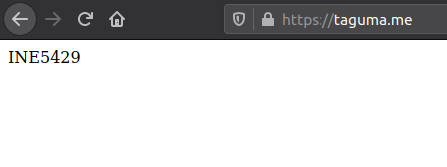
\includegraphics[width=0.8\textwidth]{seguranca.png}
    \caption{Captura de tela do dia 08/05/2021.}
\end{figure}

\end{document}
